
% Document class: article with font size 11pt
% ---------------
\documentclass[11pt,a4paper]{article}

\setlength{\textwidth}{165mm}
\setlength{\textheight}{240mm}
\setlength{\parindent}{0mm} % S{\aa} meget rykkes ind efter afsnit
\setlength{\parskip}{\baselineskip}
\setlength{\headheight}{0mm}
\setlength{\headsep}{0mm}
\setlength{\hoffset}{-2.5mm}
\setlength{\voffset}{0mm}
\setlength{\footskip}{15mm}
\setlength{\oddsidemargin}{0mm}
\setlength{\topmargin}{0mm}
\setlength{\evensidemargin}{0mm}

% Call packages
% ---------------
\usepackage{comment} %Possible to comment larger sections
%http://get-software.net/macros/latex/contrib/comment/comment.pdf
\usepackage[T1]{fontenc} %oriented to output, that is, what fonts to use for printing characters.
\usepackage[utf8]{inputenc} %allows the user to input accented characters directly from the keyboard
\usepackage[a4paper, hmargin={2.8cm, 2.8cm}, vmargin={2.5cm, 2.5cm}]{geometry}
\usepackage[super]{nth}
\PassOptionsToPackage{hyphens}{url}\usepackage{hyperref}
\usepackage{eso-pic} % \AddToShipoutPicture
\usepackage{float} % This will allow precise picture placement, use [H].
\usepackage{listings}
\usepackage{mips}
\usepackage{float}

%Support Windows TeXStudio
\usepackage[T1]{fontenc}
\usepackage{lmodern}

%http://mirrors.dotsrc.org/ctan/fonts/fourier-GUT/doc/latex/fourier/fourier-doc-en.pdf
\usepackage[english]{babel}														     % Danish
\usepackage[protrusion=true,expansion=true]{microtype}				                 % Better typography
%http://www.khirevich.com/latex/microtype/
\usepackage{amsmath,amsfonts,amsthm, amssymb}							 % Math packages
\usepackage[pdftex]{graphicx} %puts to pdf and graphic
%http://www.kwasan.kyoto-u.ac.jp/solarb6/usinggraphicx.pdf
\usepackage{xcolor,colortbl}
%http://mirrors.dotsrc.org/ctan/macros/latex/contrib/xcolor/xcolor.pdf
%http://texdoc.net/texmf-dist/doc/latex/colortbl/colortbl.pdf
\usepackage{tikz} %documentation http://www.ctan.org/pkg/pgf
\usepackage{parskip} %http://www.ctan.org/pkg/parskip
%http://tex.stackexchange.com/questions/51722/how-to-properly-code-a-tex-file-or-at-least-avoid-badness-10000
%Never use \\ but instead press "enter" twice. See second website for more info
\usepackage[font={small,it},labelfont={bf}]{caption}
% MATH -------------------------------------------------------------------
\newcommand{\Real}{\mathbb R}
\newcommand{\Complex}{\mathbb C}
\newcommand{\Field}{\mathbb F}
\newcommand{\RPlus}{[0,\infty)}
%
\newcommand{\norm}[1]{\left\Vert#1\right\Vert}
\newcommand{\essnorm}[1]{\norm{#1}_{\text{\rm\normalshape ess}}}
\newcommand{\abs}[1]{\left\vert#1\right\vert}
\newcommand{\set}[1]{\left\{#1\right\}}
\newcommand{\seq}[1]{\left<#1\right>}
\newcommand{\eps}{\varepsilon}
\newcommand{\To}{\longrightarrow}
\newcommand{\RE}{\operatorname{Re}}
\newcommand{\IM}{\operatorname{Im}}
\newcommand{\Poly}{{\cal{P}}(E)}
\newcommand{\EssD}{{\cal{D}}}
% THEOREMS ----------------------------------------------------------------
\theoremstyle{plain}
\newtheorem{thm}{Theorem}[section]
\newtheorem{cor}[thm]{Corollary}
\newtheorem{lem}[thm]{Lemma}
\newtheorem{prop}[thm]{Proposition}
%
\theoremstyle{definition}
\newtheorem{defn}{Definition}[section]
%
\theoremstyle{remark}
\newtheorem{rem}{Remark}[section]
%
\numberwithin{equation}{section}
\renewcommand{\theequation}{\thesection.\arabic{equation}}

\newfloat{code}{h}{lst}
\floatname{code}{Code}


\author{
  \Large{
    Frenzel, Sven Uhrenholdt (\href{mailto:sven@frenzel.dk}{sven@frenzel.dk}) - 130793 - cdn769}\\
}
\title{
  \huge{Compilers\\}
\vspace{3cm}
\Large{\nth{3} Weekly Assignment}
}

\begin{document}
\AddToShipoutPicture*{\put(0,0){\includegraphics*[viewport=0 0 700 600]{include/natbio-farve}}}
\AddToShipoutPicture*{\put(0,602){\includegraphics*[viewport=0 600 700 1600]{include/natbio-farve}}}

\AddToShipoutPicture*{\put(0,0){\includegraphics*{include/nat-en}}}

\clearpage\maketitle
\thispagestyle{empty}

\clearpage\newpage
\thispagestyle{plain}


\section*{Task 1}
\subsection*{Task 1.a}
\begin{code}[H]
\begin{verbatim}
LABEL l_s0
    t_1 := w
    t_2 := 0
    IF t_1 != t_2 THEN l_t0 else l_f
LABEL l_t0
    t_3 := w
    t_4 := v
    t_5 := t_3 / t_4
    t_6 := 0
    IF t_5 != t_6 THEN l_t1 else l_f
LABEL l_t1
    t_7 := w
    t_8 := v
    IF t_7 < t_8 THEN l_t2 else l_f2
LABEL l_t2
    t_9 := v
    t_10 := w
    v := t_9 - t_10
LABEL l_f2
    t_11 := w
    t_12 := v
    w := t_11 - t_12
GOTO l_s0
LABEL l_f
\end{verbatim}
\caption{Intermediate Language code for Task 1.a}
\label{code:il1a}	
\end{code}


\lstset{language=[mips]Assembler}

\begin{code}[H]
	\begin{lstlisting}
LABEL l_while
	addi $1, $1, w
	bne$1, $zero, l_true0
	jl_false
LABEL l_true0
	addi $2, $2, w
	addi $3, $3, v
	div $2, $3
	bne $LO, $zero, l_true1
	j l_false
LABEL l_true1
	addi $4, $4, w
	addi $5, $5, v
	blt $4, $5, l_true2
	j l_false2
LABEL l_true2
	addi $6, $6, v
	addi $7, $7, w
	sub v, $6, $7
	j l_while
LABEL l_false2
	addi $8, $8, w
	addi $9, $9, v
	sub w, $8, $9
	j l_while
LABEL l_false
	\end{lstlisting}
	\caption{MIPS code for Task 1.a}
    \label{code:mips1a}	
\end{code}


\subsection*{Task 1.b}
\begin{table}[H]
	\centering
	\label{my-label}
\begin{tabular}{ |l|l| }
	\hline
	\begin{minipage}{1.2in}
		\begin{verbatim}
			z := x >= y 
		\end{verbatim}
	\end{minipage} &
	\begin{minipage}{3in}
		\begin{lstlisting}
	bge   $x, $y, l_1
l_0: 
	addi  $z, $zero, 1
l_1:
	add   $z, $zero, $zero
		\end{lstlisting}
	\end{minipage} \\ \hline
	\begin{minipage}{1.2in}
		\begin{verbatim}
			w := ! z
		\end{verbatim}
	\end{minipage} &
	\begin{minipage}{3in}
		\begin{lstlisting}
	beq   $z, $zero, l_1
l_0:
	add   $w, $zero, $zero
l_1:
	addi  $w, $zero, 1
		\end{lstlisting}
	\end{minipage} \\ \hline
\end{tabular}
\caption{Patterns for MIPS}
\end{table}
\section*{Task 2}
\subsection*{Task 2.a,b,c}
\begin{table}[H]
	\centering
	\begin{tabular}{l|l|l|l|l|l|l|l|l|l|l|l|l}
		\textbf{}   & succ & gen & kill & \textbf{}   & out \#1 & in \#1 & out \#2 & in \#2 & out \#3 & in \#3 & \textbf{}   & Interference \\ \hline
		\textbf{1}  & 2    &     &      & \textbf{1}  & a,b     & a,b    & a,b     & a,b    & a,b     & a,b    & \textbf{1}  &              \\ \hline
		\textbf{2}  & 3,7  & a,b &      & \textbf{2}  & a,b     & a,b    & a,b     & a,b    & a,b     & a,b    & \textbf{2}  &              \\ \hline
		\textbf{3}  & 4    &     &      & \textbf{3}  & a,b     & a,b    & a,b     & a,b    & a,b     & a,b    & \textbf{3}  &              \\ \hline
		\textbf{4}  & 5    & a   & t    & \textbf{4}  & b,t     & a,b    & b,t     & a,b    & b,t     & a,b    & \textbf{4}  & (t,b)        \\ \hline
		\textbf{5}  & 6    & b   & a    & \textbf{5}  & a,t     & b,t    & a,t     & b,t    & a,t     & b,t    & \textbf{5}  & (a,t)        \\ \hline
		\textbf{6}  & 7    & t   & b    & \textbf{6}  & a,b     & a,t    & a,b     & a,t    & a,b     & a,t    & \textbf{6}  & (b,a)        \\ \hline
		\textbf{7}  & 8    &     &      & \textbf{7}  & a,b     & a,b    & a,b     & a,b    & a,b     & a,b    & \textbf{7}  &              \\ \hline
		\textbf{8}  & 9    &     & z    & \textbf{8}  & a,b,z   & a,b    & a,b,z   & a,b    & a,b,z   & a,b    & \textbf{8}  & (z,a),(z,b)  \\ \hline
		\textbf{9}  & 10   & a,b & b    & \textbf{9}  & a,b,z   & a,b,z  & a,b,z   & a,b,z  & a,b,z   & a,b,z  & \textbf{9}  & (b,a),(b,z)  \\ \hline
		\textbf{10} & 1,11 & b,z &      & \textbf{10} & a       & a,b,z  & a,b     & a,b,z  & a,b     & a,b,z  & \textbf{10} &              \\ \hline
		\textbf{11} & 12   &     &      & \textbf{11} & a       & a      & a       & a      & a       & a      & \textbf{11} &              \\ \hline
		\textbf{12} &      & a   &      & \textbf{12} &         & a      &         & a      &         & a      & \textbf{12} &              \\
	\end{tabular}
	\caption{succ, gen, kill, 3 sets of out and in for all instructions and interference for the program given in the assignment.}
	\label{tab:liveliness_analysis}
\end{table}
Figure \ref{fig:interference_graph} shows the interference graph based on the data computed in Table \ref{tab:liveliness_analysis}.
\begin{figure}[H]
  \centering
    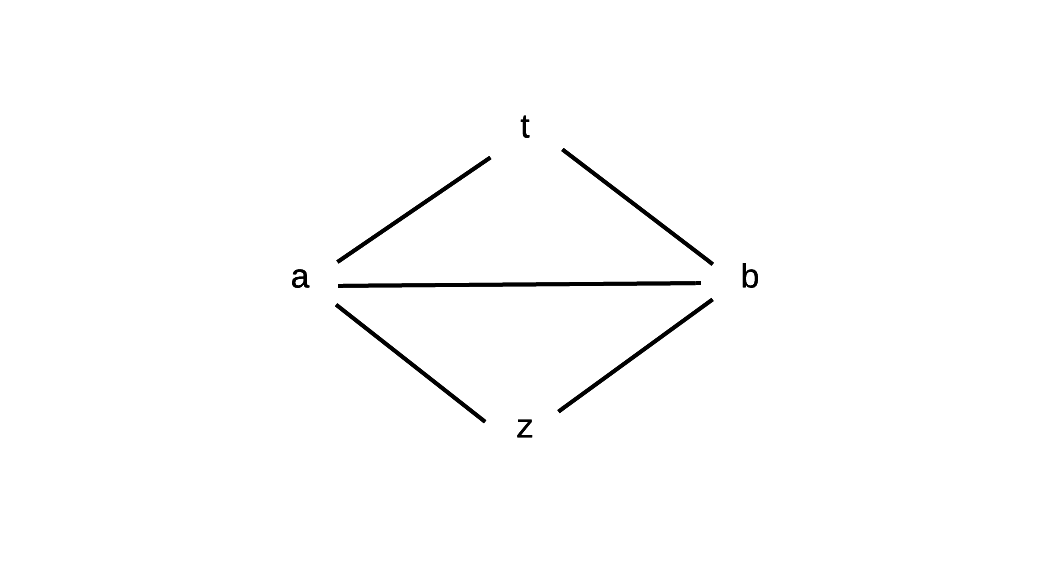
\includegraphics[width=0.5\textwidth]{fig/interference}
      \caption{Interference Graph}
      \label{fig:interference_graph}
\end{figure}
\subsection*{Task 2.d}
\begin{table}[H]
	\centering
	\begin{tabular}{l|l|l}
		b &     & 1 \\
		a & b   & 2 \\
		t & a,b & 3 \\
		z & a,b & 3
	\end{tabular}
	\caption{Stack with 3 colors.}
	\label{fig:3colorstack}
\end{table}
\subsection*{Task 2.e}
\begin{table}[H]
	\centering
	\begin{tabular}{l|l|l}
		b &     & 1 \\
		a & b   & 2 \\
		t & a,b & spill \\
		z & a,b & spill
	\end{tabular}
	\caption{Stack with 2 colors and spills.}
	\label{fig:2colorstack}
\end{table}

The Code \ref{code:codespill} shows the program from the assignment with the spills from Table \ref{fig:2colorstack}.
\begin{code}[H]
\begin{verbatim}
     gcd(a,b) {
     1:  LABEL start
     2:  IF a < b THEN next ELSE swap
     3:  LABEL swap
     4:  t_4  := a
         M[address_t] := t_4
     5:  a    := b
         t_6  := M[address_t]
     6:  b    := t_6
     7:  LABEL next
     8:  z_8  := 0
         M[address_z] := z_8
     9:  b    := b mod a
         z_10 := M[address_z]
     10: IF b = z_10 THEN end ELSE start
     11: LABEL end
     12: RETURN a
     }
\end{verbatim}
\caption{Program from Task 2 after spilling.}
\label{code:codespill}	
\end{code}
\end{document}